%30/01 - Raúl Guantes
\chapter{Conceptos básicos}
\section{La importancia de cuantificar y estimar las escalas en biología}
La biología de sistemas es un campo que busca entender los sistemas biológicos a través de la cuantificación y la modelización matemática. Los modelos matemáticos son simplificaciones de sistemas biológicos complejos, y aunque no son perfectos (ya que no pueden capturar toda la información), son útiles para entender y predecir comportamientos biológicos. Como dijo el estadístico George Box: "Todos los modelos son erróneos, pero algunos son útiles".

Una herramienta clave en este campo es BioNumbers, una base de datos que recopila información cuantitativa en biología. Esta información es esencial para interpretar resultados experimentales y diseñar nuevos experimentos. Por ejemplo, al realizar experimentos, es fundamental calcular la media y la desviación estándar de los resultados para estimar el error. El error se redondea a una cifra significativa, y la medida se expresa con la misma precisión que el error.

\subsection{Estimación de la expresión de proteínas en \textit{E. coli}}
Supongamos que encontramos una proteína en un cultivo celular de \textit{E. coli} con una concentración de 1 picoMolar (pM) por célula. ¿Es esta expresión significativa? Para responder, necesitamos calcular el número de moléculas de la proteína por célula, lo que depende del volumen celular.

\paragraph{Datos} Las bacterias tienen forma cilíndrica con una longitud de 2 micras y un diámetro de 1 micra. La concentración de la proteína: $C = 1 pM = 10^{-12}M$.

\paragraph{Cálculos}
\begin{enumerate}
\item Volumen de la célula
$$V = \pi r^2 h \rightarrow \pi (0,5 \mu m)^2 2 \approx 1,5 \mu m^3 = 1,5 \cdot 10^{-15} l = 1,5 fl$$
\item Número de moléculas de proteína por célula
$$C = \frac{N_p}{V \cdot N_{av}} \rightarrow N_p = C \cdot V \cdot N_{av}$$
$$N_p = C \cdot V \cdot N_{av} = 10^{-12}M \cdot 1,5 \cdot 10^{-15}l \cdot 6 \cdot 10^{23} \approx 10^{-3} molecules$$
Esto significa que hay aproximadamente 1 molécula de proteína por cada 1.000 células.
\end{enumerate}

De esta forma, podemos decir que como regla general, una concentración de 1 nanomolar (nM) en \textit{E. coli} corresponde aproximadamente a 1 molécula por célula, dado que el volumen de una célula de \textit{E. coli} es del orden de 1 fl.

\subsection{Variabilidad en la cuantificación de proteínas}
En \textit{E. coli}, la cantidad de proteínas se ha cuantificado utilizando dos técnicas principales: espectrometría de masas y microscopía de fluorescencia. Estas técnicas arrojan resultados diferentes:
\begin{itemize}
\item En espectrometría de masas, el número promedio de una proteína cualquiera en \textit{E. coli} es de 1.000-2.000 moléculas.
\item En microscopía de fluorescencia, este número es de alrededor de 50 moléculas.
\end{itemize}

\begin{figure}[h]
\centering
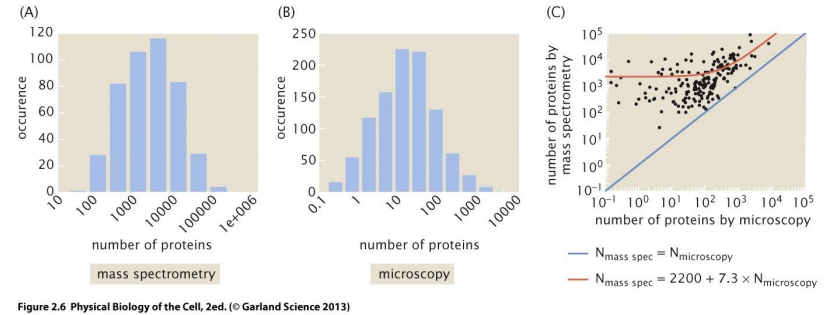
\includegraphics[width = 0.9\textwidth]{figs/mol-census.png}
\end{figure}

Para \textbf{proteínas muy abundantes}, ambas técnicas muestran una buena correlación.
Para \textbf{proteínas poco abundantes}, la correlación se pierde debido a la variabilidad intrínseca en la expresión génica. Esto no es un artefacto experimental, sino una consecuencia de la estocasticidad en los procesos biológicos (limitación física). Cuando el número de copias de una proteína es bajo, la probabilidad de que ocurran reacciones bioquímicas al azar es menor. Esto genera una gran variabilidad en la cantidad de proteínas entre células genéticamente idénticas. En cambio, cuando el número de copias es alto, las reacciones ocurren con mayor frecuencia, reduciendo la variabilidad.

\subsection{Consecuencias numéricas en biología}
La expresión génica es un proceso altamente estocástico debido al bajo número de copias de muchas moléculas involucradas (ADN, factores de transcripción, ARN polimerasa, etc.). Esto tiene varias implicaciones:
\begin{itemize}
\item \textbf{Variabilidad celular:} Incluso en poblaciones de células clonales en el mismo ambiente, la expresión de proteínas varía significativamente. Por ejemplo, las huellas dactilares de dos gemelos son diferentes debido a esta variabilidad.
\item \textbf{Estocasticidad como mecanismo evolutivo:} La aleatoriedad en la expresión génica puede ser aprovechada para generar diversidad. Por ejemplo, en \textit{Bacillus subtilis}, algunas células entran en estado de esporulación en ausencia de nutrientes, mientras que otras continúan dividiéndose.
\end{itemize}

\subsection{Ejemplo: distancia media entre proteínas en una célula de \textit{E. coli}}
La distancia entre proteínas en una célula es inversamente proporcional a la concentración de proteínas (a mayor concentración de proteínas, menos distancia entre ellas). Matemáticamente, siendo c la concentración de proteínas:
$$c = \frac{1}{V_b} = \frac{1}{d^3} \rightarrow d \approx \frac{1}{c^{\frac{1}{3}}}$$

Los cálculos serían los siguientes:
\begin{enumerate}
\item Concentración total de proteínas en \textit{E. coli}:
$$c_{\text{total protein}} = \frac{N^T_p}{V_{E.coli}}$$
\begin{itemize}
\item Peso de \textit{E. coli}: 1 pg. De ahí, el 70\% es agua y el 30\% es masa seca. Las proteínas equivalen al 50\% de la masa seca. Masa total de proteínas en \textit{E. coli}: $0,15 pg = 15 \cdot 10^{-14} g$
\item Sabemos que una proteína tiene de media 300 aminoácidos, y que cada aminoácido tiene una masa media de 100 Dalton. Por tanto, una proteína tiene de media  $3 \cdot 10^4$ Dalton. Un Dalton son $1,7 \cdot 10^{-24}$ gramos. Así:
$$3\cdot 10^4 \cdot 1,7 \cdot 10^{-24} \approx 5 \cdot 10^{-20}$$. 

Masa promedio de una proteína: $5 \cdot 10^{-20} g$

\item Número total de proteínas:
$$N^T_p = \frac{\text{masa total de prot en E. coli}}{\text{masa promedio de 1 proteina}} \rightarrow \frac{15 \cdot 10^{-14}}{5 \cdot 10^{-20}} = 3 \cdot 10^6$$
\item Concentración:
$$c_{\text{total protein}} = \frac{3 \cdot 10^6}{10^9} = 3 \cdot 10^{-3} mol/cel$$
\end{itemize}
\item Distancia media entre proteínas:
$$d = \frac{1}{(3 \cdot 10^{-3})^{\frac{1}{3}}} \approx 7nm$$
\end{enumerate}

El radio típico de una proteína en \textit{E. coli} es de 2-5 nm. Una distancia media de 7 nm indica que las proteínas están muy cerca unas de otras, un fenómeno conocido como "\textbf{molecular crowding}".
Este hacinamiento molecular tiene consecuencias físicas: muchas reacciones bioquímicas están limitadas por la \textbf{difusión lenta} de las moléculas. Por ello, las células han desarrollado estructuras como los microtúbulos para facilitar el transporte y la movilidad, y las constantes de reacción medidas \textit{in vitro} no son iguales a las medidas \textit{in vivo}

\section{Dinámicas en biología}
Los sistemas biológicos son dinámicos, es decir, cambian con el tiempo. Estos cambios pueden ocurrir a diferentes escalas temporales, desde milisegundos hasta años, y son fundamentales para entender cómo funcionan los organismos. Por ejemplo, las células responden a señales externas (como nutrientes o estrés) codificando información en la amplitud, duración y frecuencia de estas señales.

Los sistemas dinámicos en biología se modelan con \textbf{ecuaciones diferenciales}, que describen cómo cambian las variables biológicas (como la concentración de proteínas) en el tiempo. Estas ecuaciones capturan la velocidad de cambio de una variable en función de otras variables. Por ejemplo, si $P(t)$ es la cantidad de una proteína en el tiempo $t$, su dinámica se describe como:
$$\frac{dP}{dt} = f(P, ARN, TF, ...)$$
donde $dP/dt$ es la velocidad de cambio de la proteína y $f(P, ARN, TF)$ una función dependiente de la proteína P, el ARN, los factores de transcripción TF, y otros factores.

Para la interpretación de la derivada $dP/dt$ se tiene en cuenta:
\begin{itemize}
\item Si $dP/dt > 0$: la proteína aumenta con el tiempo.
\item Si $dP/dt < 0$: la proteína disminuye con el tiempo.
\item Si $dP/dt > 1$: el cambio es rápido.
\item Si $dP/dt < 1$: el cambio es lento.
\end{itemize}

La función genérica es: $\frac{dP}{dt} = f(u, t; \mu)$, siendo $u$ las variables dinámicas, $\mu$ los parámetros y $u(t)$ las trayectorias o soluciones. Para esto, es importante especificar las \textbf{condiciones iniciales}. Si todas las variables en $f$ tienen exponente 1, el sistema es \textbf{lineal}. Si alguna variable tiene un exponente mayor que 1, el sistema es \textbf{no lineal}.

\subsection{Sistemas deterministas vs estocásticos}
Las ecuaciones diferenciales ordinarias (EDOs) describen sistemas \textbf{deterministas}, donde el comportamiento es predecible y continuo en el tiempo (homogéneo). Sin embargo, en biología, muchos sistemas son \textbf{estocásticos} (aleatorios) debido a fluctuaciones intrínsecas. Por ejemplo, en un experimento de apoptosis en células tumorales:
\begin{itemize}
\item Las proteínas marcadas con fluorescencia muestran fluctuaciones individuales en el tiempo.
\item Las simulaciones deterministas capturan el promedio poblacional, pero no las variaciones individuales.
\end{itemize}

\begin{figure}[h]
\centering
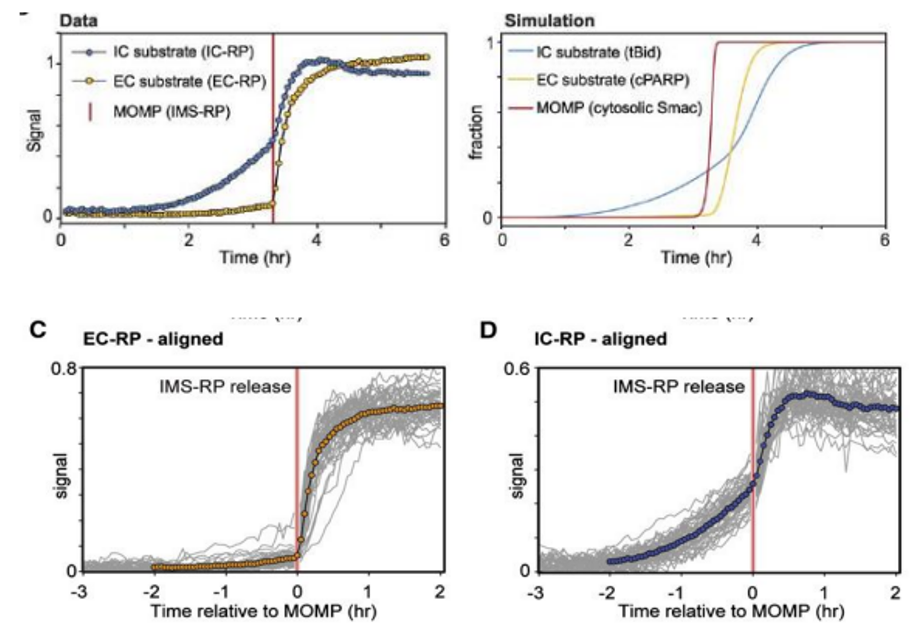
\includegraphics[width = 0.6\textwidth]{figs/simul-cells.png}
\end{figure}

En el artículo se ha estudiado el proceso de apoptosis de células tumorales tras administrar una droga (un fármaco). Las proteínas se han marcado fluorescentemente, y se puede ver cómo cambian las distintas proteínas tras la administración. Esto se puede simular de forma precisa, pero estas simulaciones se corresponden a experimentos de los que se obtiene una media poblacional. Las proteínas individuales tienen fluctuaciones en el tiempo. Todas las fluctuaciones están promedidadas, por lo que el modelo de ecuaciones diferenciales determinista simula el promedio de las células. En los experimentos se mide la fluorescencia total en la célula, no su localización subcelular.

En algunos sistemas, como el desarrollo embrionario, las \textbf{coordenadas espaciales} son cruciales. Las células se diferencian según su posición, y los genes se expresan en "oleadas". Para modelar estos sistemas, se usan \textbf{ecuaciones diferenciales parciales (EDPs),} que consideran tanto el tiempo como el espacio.

\begin{figure}[h]
\centering
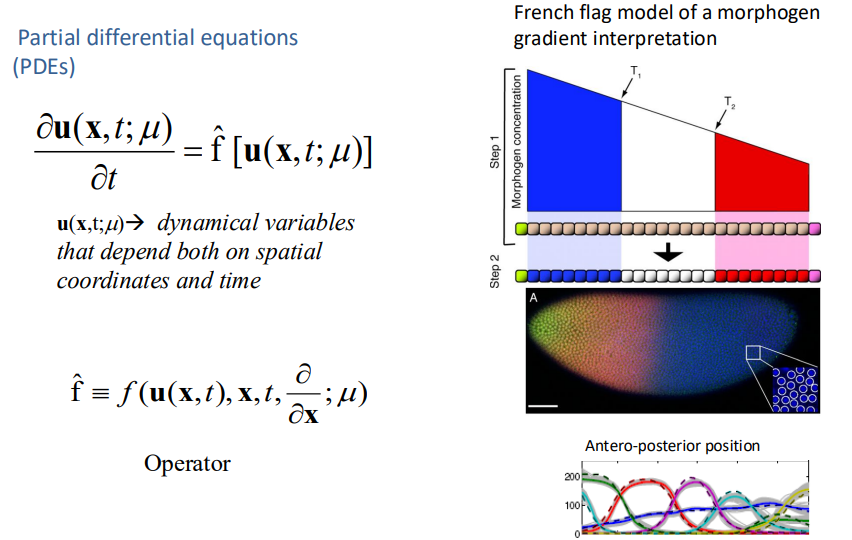
\includegraphics[width = 0.6\textwidth]{figs/pde-embryo.png}
\end{figure}

\section{Procesos dinámicos simples celulares: crecimiento celular, dilución proteica y degradación}
\subsection{Crecimiento celular}
El crecimiento celular es un proceso dinámico donde el número de células $N(t)$ aumenta con el tiempo. La velocidad de crecimiento se describe con la ecuación:
$$\frac{dN}{dt} = rN$$
donde r es la tasa de crecimiento y $N(t)$ el número de células en el tiempo t. Se trata de un sistema lineal con una sola variable. Los pasos para resolver la ecuación son:
\begin{enumerate}
\item Separar variables:
$$\frac{dN}{N} = r dt$$
\item Integrar ambos lados:
$$\int \frac{dN}{N} = \int r \cdot dt \rightarrow ln N = r t + C$$
\item Aplicar exponencial
$$N(t) = e^{rt + C} = e^C \cdot e^{rt}$$
\item Definir la constante $e^C = N(0)$, el número inicial de células o condiciones iniciales:
$$N(t) = N(0) \cdot e^{rt}$$
\end{enumerate}

El tiempo de duplicación $T_{div}$ indica el tiempo necesario para que $N(t)$ se duplique. Se calcula como:
$$N(T_{div}) = 2N(0) = N(0) \cdot e^{r \cdot T_{div}}$$
Dividiendo por $N(0)$:
$$ e^{r \cdot T_{div}} = 2 \rightarrow r \cdot T_{div} = ln 2 \rightarrow r = \frac{ln 2}{T_{div}}$$

\subsection{Dilución proteica}
Durante el crecimiento celular, las proteínas se diluyen debido al aumento del volumen celular. Si $P(t)$ es la cantidad de una proteína, su dinámica se describe como:
$$\frac{dP}{dt} = rP - \frac{P}{T_{div}}$$

\subsection{Degradación proteica}
Las proteínas también se degradan con una tasa constante $k_d$. La dinámica se describe como:
$$\frac{dP}{dt} = -k_dP \rightarrow P(t) = P(0) \cdot e^{-k_dt}$$

\subsection{Combinación de procesos}
En una célula, el crecimiento, la dilución y la degradación ocurren simultáneamente. La dinámica combinada se describe como:
$$\frac{dP}{dt} = rP - \frac{P}{T_{div}} - k_dP$$
Esta ecuación captura cómo cambia la proteína debido al crecimiento, la dilución y la degradación.

\subsection{Ejercicio: Malthusian growth of bacteria}
Con el modelo lineal de crecimiento celular, ¿cuánto tiempo tardará una sola bacteria que se divide a un ritmo constante en llenar todos los océanos del mundo?. Datos: Supongamos que las bacterias tienen un volumen de 1 micrómetro cúbico y se dividen cada 30 minutos (valores típicos en \textit{E. coli}). El volumen estimado de todos los océanos es de $292.131.000 km^3$.

Tenemos los siguientes datos:
$$V_{oceans} = 300.000.000 km^3 = 3 \cdot 10^8 km^3 = 3 \cdot 10^8 \cdot 10^{27} \mu m^3 = 3 \cdot 10^{35} \mu m^3$$
$$V_{bac} = 1 \mu m$$
$$T_{div} = 30 mins = 0,5 h$$
$$c_0 = 1$$

$$r = \frac{ln 2}{30 min} = 0.023$$
$$N(t) = 1 \cdot e^{0.023 \cdot t}$$

$$N = V_o / V_b$$

$$3 \cdot 10^{35} = e^{\frac{ln 2}{0,5} \cdot t} \rightarrow ln 3 + 35 \cdot ln 10 = \frac{ln 2}{0,5} \cdot t \rightarrow t = 58 h$$

Este modelo no es útil porque está demasiado simplificado. Hay que tener en cuenta los nutrientes, las restricciones espaciales, etc. 